\documentclass[tikz,border=10pt]{standalone}
\usepackage{pgfplots}
\pgfplotsset{compat=1.18}

\begin{document}

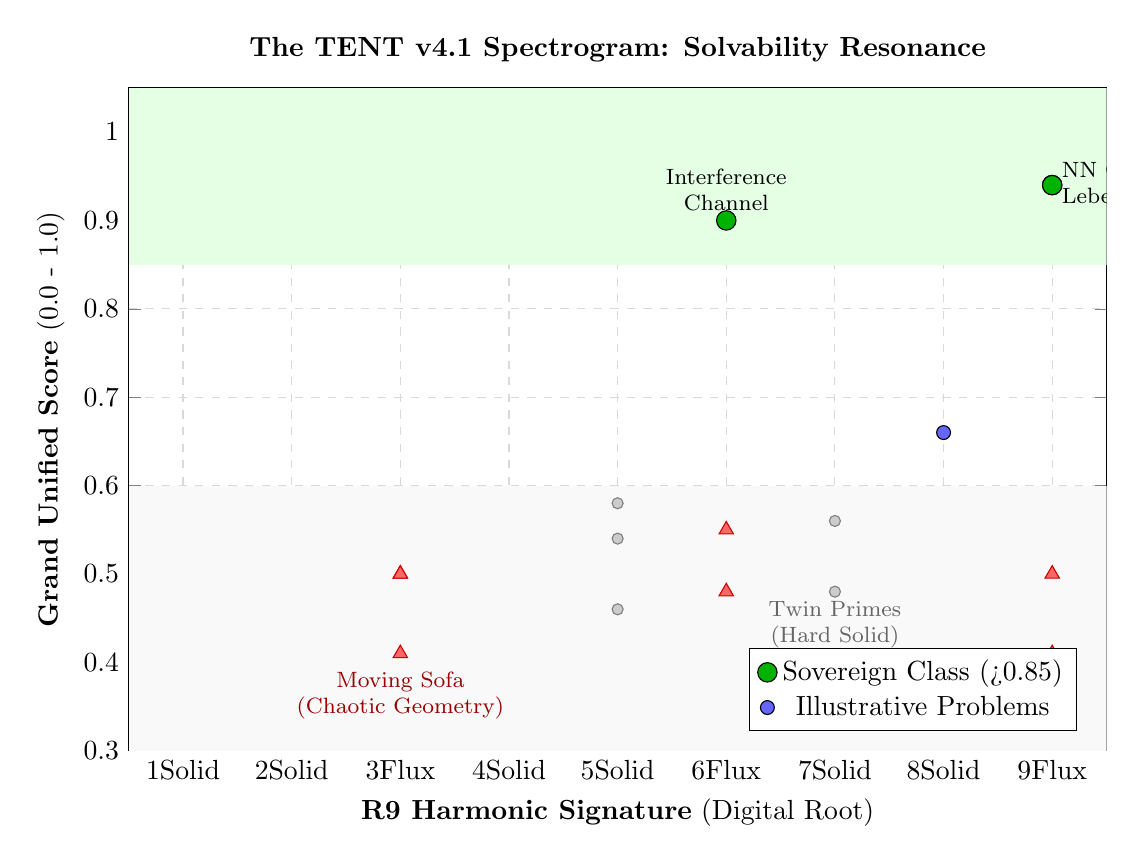
\begin{tikzpicture}
    \begin{axis}[
        title={\textbf{The TENT v4.1 Spectrogram: Solvability Resonance}},
        xlabel={\textbf{R9 Harmonic Signature} (Digital Root)},
        ylabel={\textbf{Grand Unified Score} (0.0 - 1.0)},
        xmin=0.5, xmax=9.5,
        ymin=0.3, ymax=1.05,
        xtick={1,2,3,4,5,6,7,8,9},
        xticklabels={1\\Solid, 2\\Solid, 3\\Flux, 4\\Solid, 5\\Solid, 6\\Flux, 7\\Solid, 8\\Solid, 9\\Flux},
        ytick={0.3, 0.4, 0.5, 0.6, 0.7, 0.8, 0.9, 1.0},
        grid=major,
        major grid style={dashed, gray!30},
        scatter/classes={
            solved={mark=*, mark size=3.5pt, draw=black, fill=green!70!black},
            probable={mark=*, mark size=2.5pt, draw=black, fill=blue!60},
            hard={mark=*, mark size=2.0pt, draw=gray, fill=gray!40},
            flux={mark=triangle*, mark size=3pt, draw=red!80!black, fill=red!60}
        },
        legend pos=south east,
        width=14cm,
        height=10cm
    ]

    % --- ZONE: THE SOVEREIGN CLUSTER (SOLVED) ---
    \fill[green!10] (axis cs:0.5, 0.85) rectangle (axis cs:9.5, 1.05);
    \node[anchor=south] at (axis cs:5, 1.05) {\textbf{\textit{The Sovereign Zone (3.7\% Solvability)}}};

    % --- ZONE: THE CHAOS FLOOR (HARD) ---
    \fill[gray!5] (axis cs:0.5, 0.3) rectangle (axis cs:9.5, 0.60);

    % --- DATA POINTS (Subset of The Gauntlet) ---
    
    % SOLVED (The Anchor Tenants)
    \addplot[scatter, only marks, scatter src=explicit symbolic]
    coordinates {
        (9, 0.94) [solved] % Neural Networks (R9=9)
        (9, 0.94) [solved] % Lebesgue Universal Covering (R9=9)
        (6, 0.90) [solved] % Interference Channel (R9=6)
        (8, 0.66) [probable] % Landau's Problems (Borderline)
    };

    % FLUX / HARD (Illustrative Examples)
    \addplot[scatter, only marks, scatter src=explicit symbolic]
    coordinates {
        % R9 = 3 (Flux)
        (3, 0.50) [flux] % Lonely Runner
        (3, 0.41) [flux] % Moving Sofa
        (3, 0.50) [flux] % KdV Extensions
        
        % R9 = 6 (Flux)
        (6, 0.55) [flux] % Qualia Inversion
        (6, 0.48) [flux] % Chromatic Number Plane
        
        % R9 = 9 (Flux/Source)
        (9, 0.41) [flux] % Smooth 4D Poincaré
        (9, 0.50) [flux] % Cosmological Constant
        
        % R9 = 5 (Solid - The Struggle Zone)
        (5, 0.54) [hard] % Birch & Swinnerton-Dyer
        (5, 0.58) [hard] % Graph Isomorphism
        (5, 0.46) [hard] % One-Way Functions
        
        % R9 = 7 (Solid - Prime Mystery)
        (7, 0.48) [hard] % Twin Prime
        (7, 0.56) [hard] % Perfect Cuboid
    };

    % --- ANNOTATIONS ---
    \node[anchor=west, align=left, font=\footnotesize] at (axis cs: 9, 0.94) {NN Generalization \\ Lebesgue Covering};
    \node[anchor=south, align=center, font=\footnotesize] at (axis cs: 6, 0.90) {Interference\\Channel};
    
    \node[anchor=north, align=center, font=\footnotesize, color=red!60!black] at (axis cs: 3, 0.40) {Moving Sofa\\(Chaotic Geometry)};
    \node[anchor=north, align=center, font=\footnotesize, color=gray!80!black] at (axis cs: 7, 0.48) {Twin Primes\\(Hard Solid)};

    % Legend
    \legend{Sovereign Class (>0.85), Illustrative Problems}

    \end{axis}
\end{tikzpicture}

\end{document}
